\section*{Control}

Now that a functioning simulation environment is created a control hierarchy is needed. The initial thought is a multivariable control on top on single joint control. The multivariable control is done in Python or Matlab. The multivariable control will use the joint positions and joint velocities to compute the desired joint torques which is sent to joint PID controllers which is handled by using ROS control package. The first thing to do is therefore to create the individual joint PID controllers. 
To create these controllers two new files are needed. A new launch file must be created. It is possible to just append the launch file for Gazebo, but to make everything more understandable and if the package is to be used on the real robot it is easiest to make a new launch file that can be included in other launch files. The task of the control.launch file is to spawn a node which spawns all of the five controllers as 
\begin{lstlisting}[language=xml,caption={Spawns the controller node}\label{lst:launchControl}]
  <node name="controller_spawner" pkg="controller_manager" type="spawner" respawn="false"
	output="screen" ns="/five_dof_robotarm" args="joint_state_controller
                                                base_to_turntable_controller
                                                second_joint_controller
                                                third_joint_controller
                                                fourth_joint_controller
                                                fifth_joint_controller"/>
\end{lstlisting}


The other file to be created is a .yaml file which is an configuration file stat states the PID parameters and what kind of controller it is. For our example the controller will be an effort controller which is a torque controller. To be able to steer the robot in Gazebo it is needed to add a transmission object for each of the joints to be controlled in the URDF file. This object can be viewed in \lstref{lst:urdfcontrol}

\begin{lstlisting}[language=xml,caption={Controller object in the URDF file}\label{lst:urdfcontrol}]
<transmission name="joint2">
  <type>transmisson_interface/SimpleTransmission</type>
  <actuator name="joint2_motor">
  <!--mechanicalReduction>1</mechanicalReduction-->
  </actuator>
  <joint name="second_motor_to_first_bracket">
    <hardwareInterface>hardware_interface/EffortJointInterface</hardwareInterface>
  </joint>
</transmission>
\end{lstlisting}




A Gazebo element is also needed in the URDF file such that we dynamically link to the ROS library which will tell Gazebo what tot do. This way it is easy to interact with Gazebo via ROS. 


\subsection*{Connect with ROS via Python and Matlab}
What we now have done is to create a robot model described by an URDF file which we can spawn in the simulation environment Gazebo. To do control on the robot we need to know the jointpositions and joint velocites. It must also be possible to send the desired joint torques to the controllers that were specified in the yaml file. 

\subsubsection*{Python}
To communicate with the robot we need one subscriber that will listen to the joint state topic that publishes among other things the joint positions and joint velocities. 





\subsection*{PD controller with gravity compensation}
    The first controller that is going to be tested is a simple PD controller with gravity compensation:
    $$
        u=K_p\tilde{q} - K_d\dot{q} +g(q)
    $$
     where $\tilde{q} = q_d - q$ and 
     \begin{align}\label{eq:gravity}
     g(q) = \frac{\partial P}{\partial q_k}
     \end{align}

     
     and the total potential energy for a n-link robot is $P = \sum^n_{i=1}P_i$. Where $P_i$ is the potential energy for each individual link. For this specific manipulator the center of mass is assumed in the geometric center of each link. 
     \\
     Using figure \figref{draw:pot-rob} to calculate the potential energies:

     
     \begin{align*}
        P_1 &= 0
        \\
        P_2 &= m_2g\frac{L_2}{2}\sin{(q_2)}
        \\
        P_3 &= m_3g\left( L_2 \sin{(q_2)} + \frac{L_3}{2}\sin{(q_2 + q_3)} \right)
        \\
        P_4 &= m_4g\left( L_2 \sin{(q_2)} + L_3\sin{(q_2 + q_3)} + \frac{L_4}{2}\sin{(q_2+q_3+q_4)} \right)
        \\
        P_5 &= m_5g\left( L_2 \sin{(q_2)} + L_3\sin{(q_2 + q_3)} + \left(L_4 + \frac{L_5}{2} \right)\sin{(q_2+q_3+q_4)} \right)
        \\
        P &= P_1 + P_2 + P_3 + P_4 + P_5
     \end{align*}

     $L_4$ is the part up to the rotational joint. $L_5$ and $m_5$ is the rotational joint and the gripper together. To calculate individual gravity components we are using \eqref{eq:gravity}

     \begin{align*}
        g_1 &= 0
        \\
        g_2 &= \frac{\partial P}{\partial q_2} = 
        m_2g\frac{L_2}{2}\cos{(q_2)}+
        m_3g\left( L_2 \cos{(q_2)} + \frac{L_3}{2}\cos{(q_2+q_3)} \right)\\&+
        m_4g\left( L_2 \cos{(q_2)} + L_3\cos{(q_2 + q_3)} + \frac{L_4}{2}\cos{(q_2+q_3+q_4)} \right)\\&+
        m_5g\left( L_2 \cos{(q_2)} + L_3\cos{(q_2 + q_3)} + \left(L_4 + \frac{L_5}{2} \right)\cos{(q_2+q_3+q_4)} \right)
        \\
        g_3 &= \frac{\partial P}{\partial q_3} =
        m_3g\frac{L_3}{2}\cos{(q_2+q_3)} +
        m_4g\left( L_3\cos{(q_2 + q_3)} + \frac{L_4}{2}\cos{(q_2+q_3+q_4)} \right)\\&+
        m_5g\left(  L_3\cos{(q_2 + q_3)} + \left(L_4 + \frac{L_5}{2} \right)\cos{(q_2+q_3+q_4)} \right)
        \\
        g_4 &=\frac{\partial P}{\partial q_4} = 
        m_4g\frac{L_4}{2}\cos{(q_2+q_3+q_4)}+
        m_5g\left(L_4 + \frac{L_5}{2} \right)\cos{(q_2+q_3+q_4)}
        \\
        g_5 &= 0
        \\
        g(q) &= [g_1,g_2,g_3,g_4,g_5]^T
     \end{align*}

NOTE to self: Since the manipulator zero position is straight upwards this calculation is wrong. Replace sin with cos and vice versa. Remember signs. 

\begin{figure}[htbp]
    \centering
    \input{tex/drawing/robotarm.tex}
    \caption{Figure of the robot. The twisting joints are left out}
    \label{draw:pot-rob}
\end{figure}


\subsection*{Tests with step response.}
In \figref{fig:testkp1} and \figref{fig:testkp2} the step response for the joint angles are plotted. \figref{fig:testkp1} is the joint angles when $kp = 1$ for the rotational joints ($q_2$ to $q_4$) and $kp = 1.5$ for the twist joints.  \figref{fig:testkp2} is the joint angles when $kp = 2$ for the rotational joints and $kp = 1.5$ for the twist joints. From the plots one can see that with a $kp$ bigger than $2$ will lead to unwanted oscillations. $kp = 1$ looks like the best choice for this controller so far. Keep in mind that this is the step response. The next step will be to make a spline to such that the steps are not so big. $kd = 0.9$ for the rotational joints bigger than this will cause weird oscillations.

\begin{figure}[htbp]
  \centering
  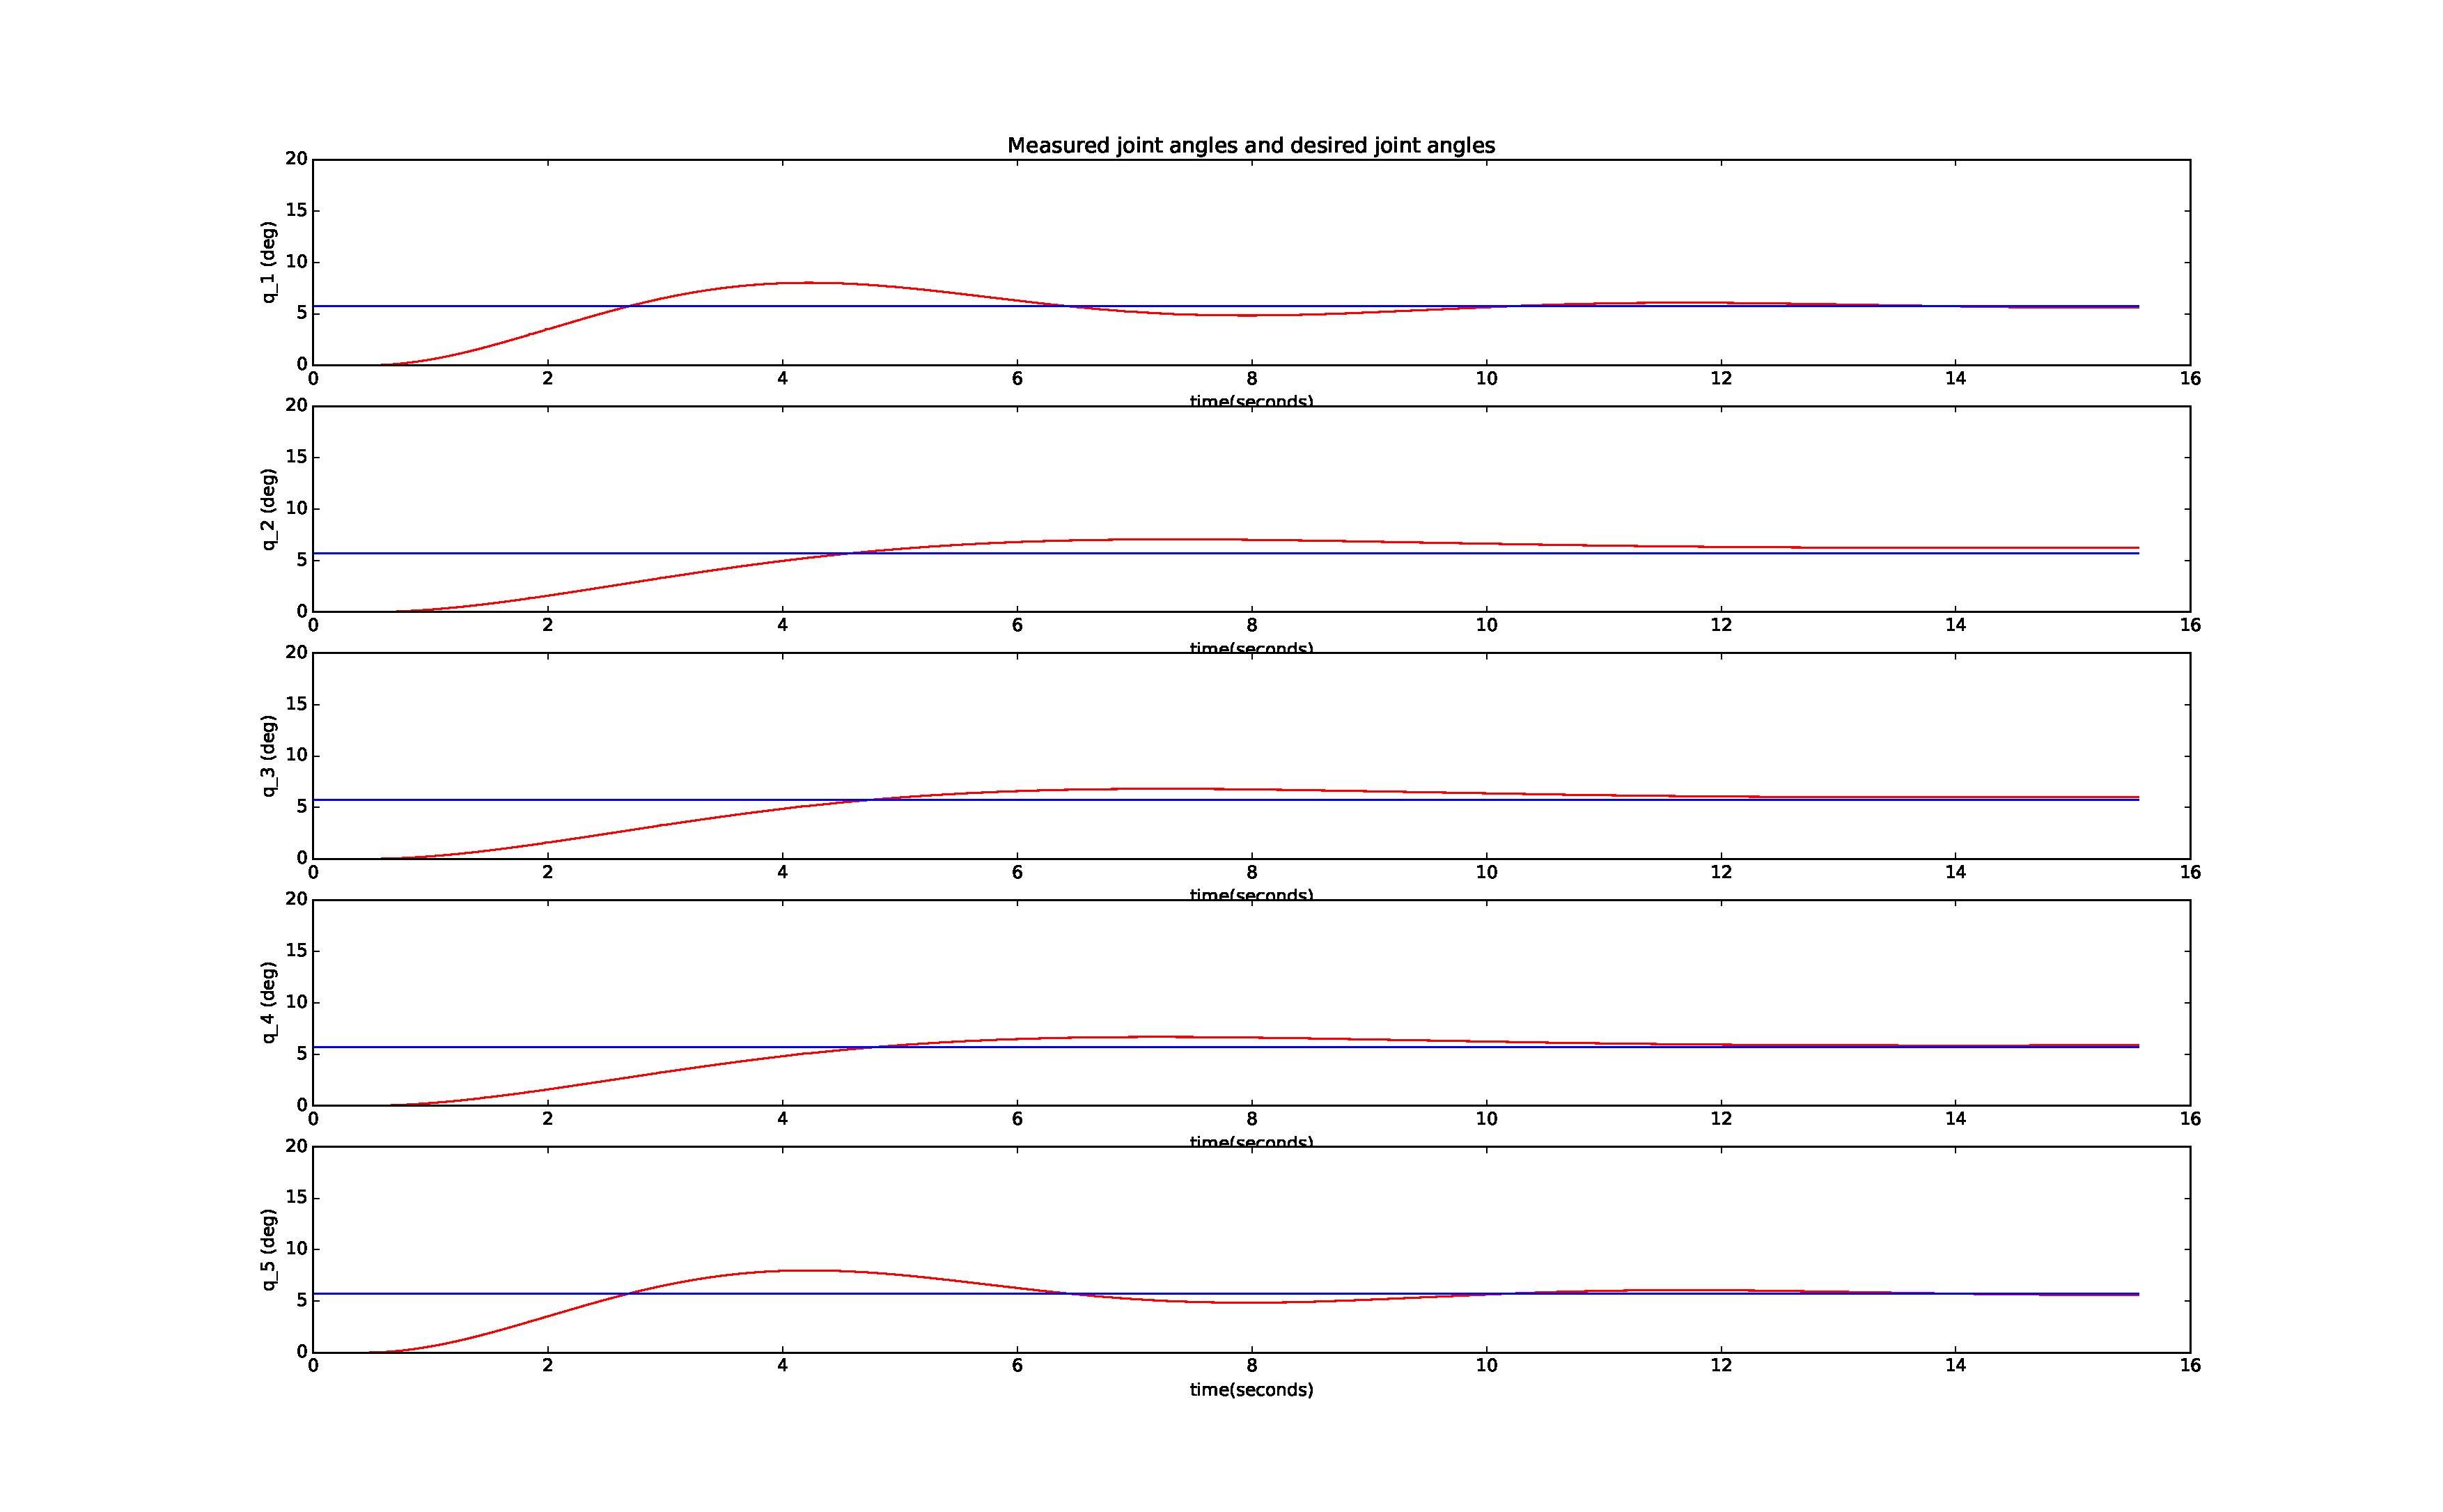
\includegraphics[width=.9\textwidth]{img/joingangKp1.eps}
  \caption{}
  \label{fig:testkp1}
\end{figure}
\begin{figure}[htbp]
  \centering
  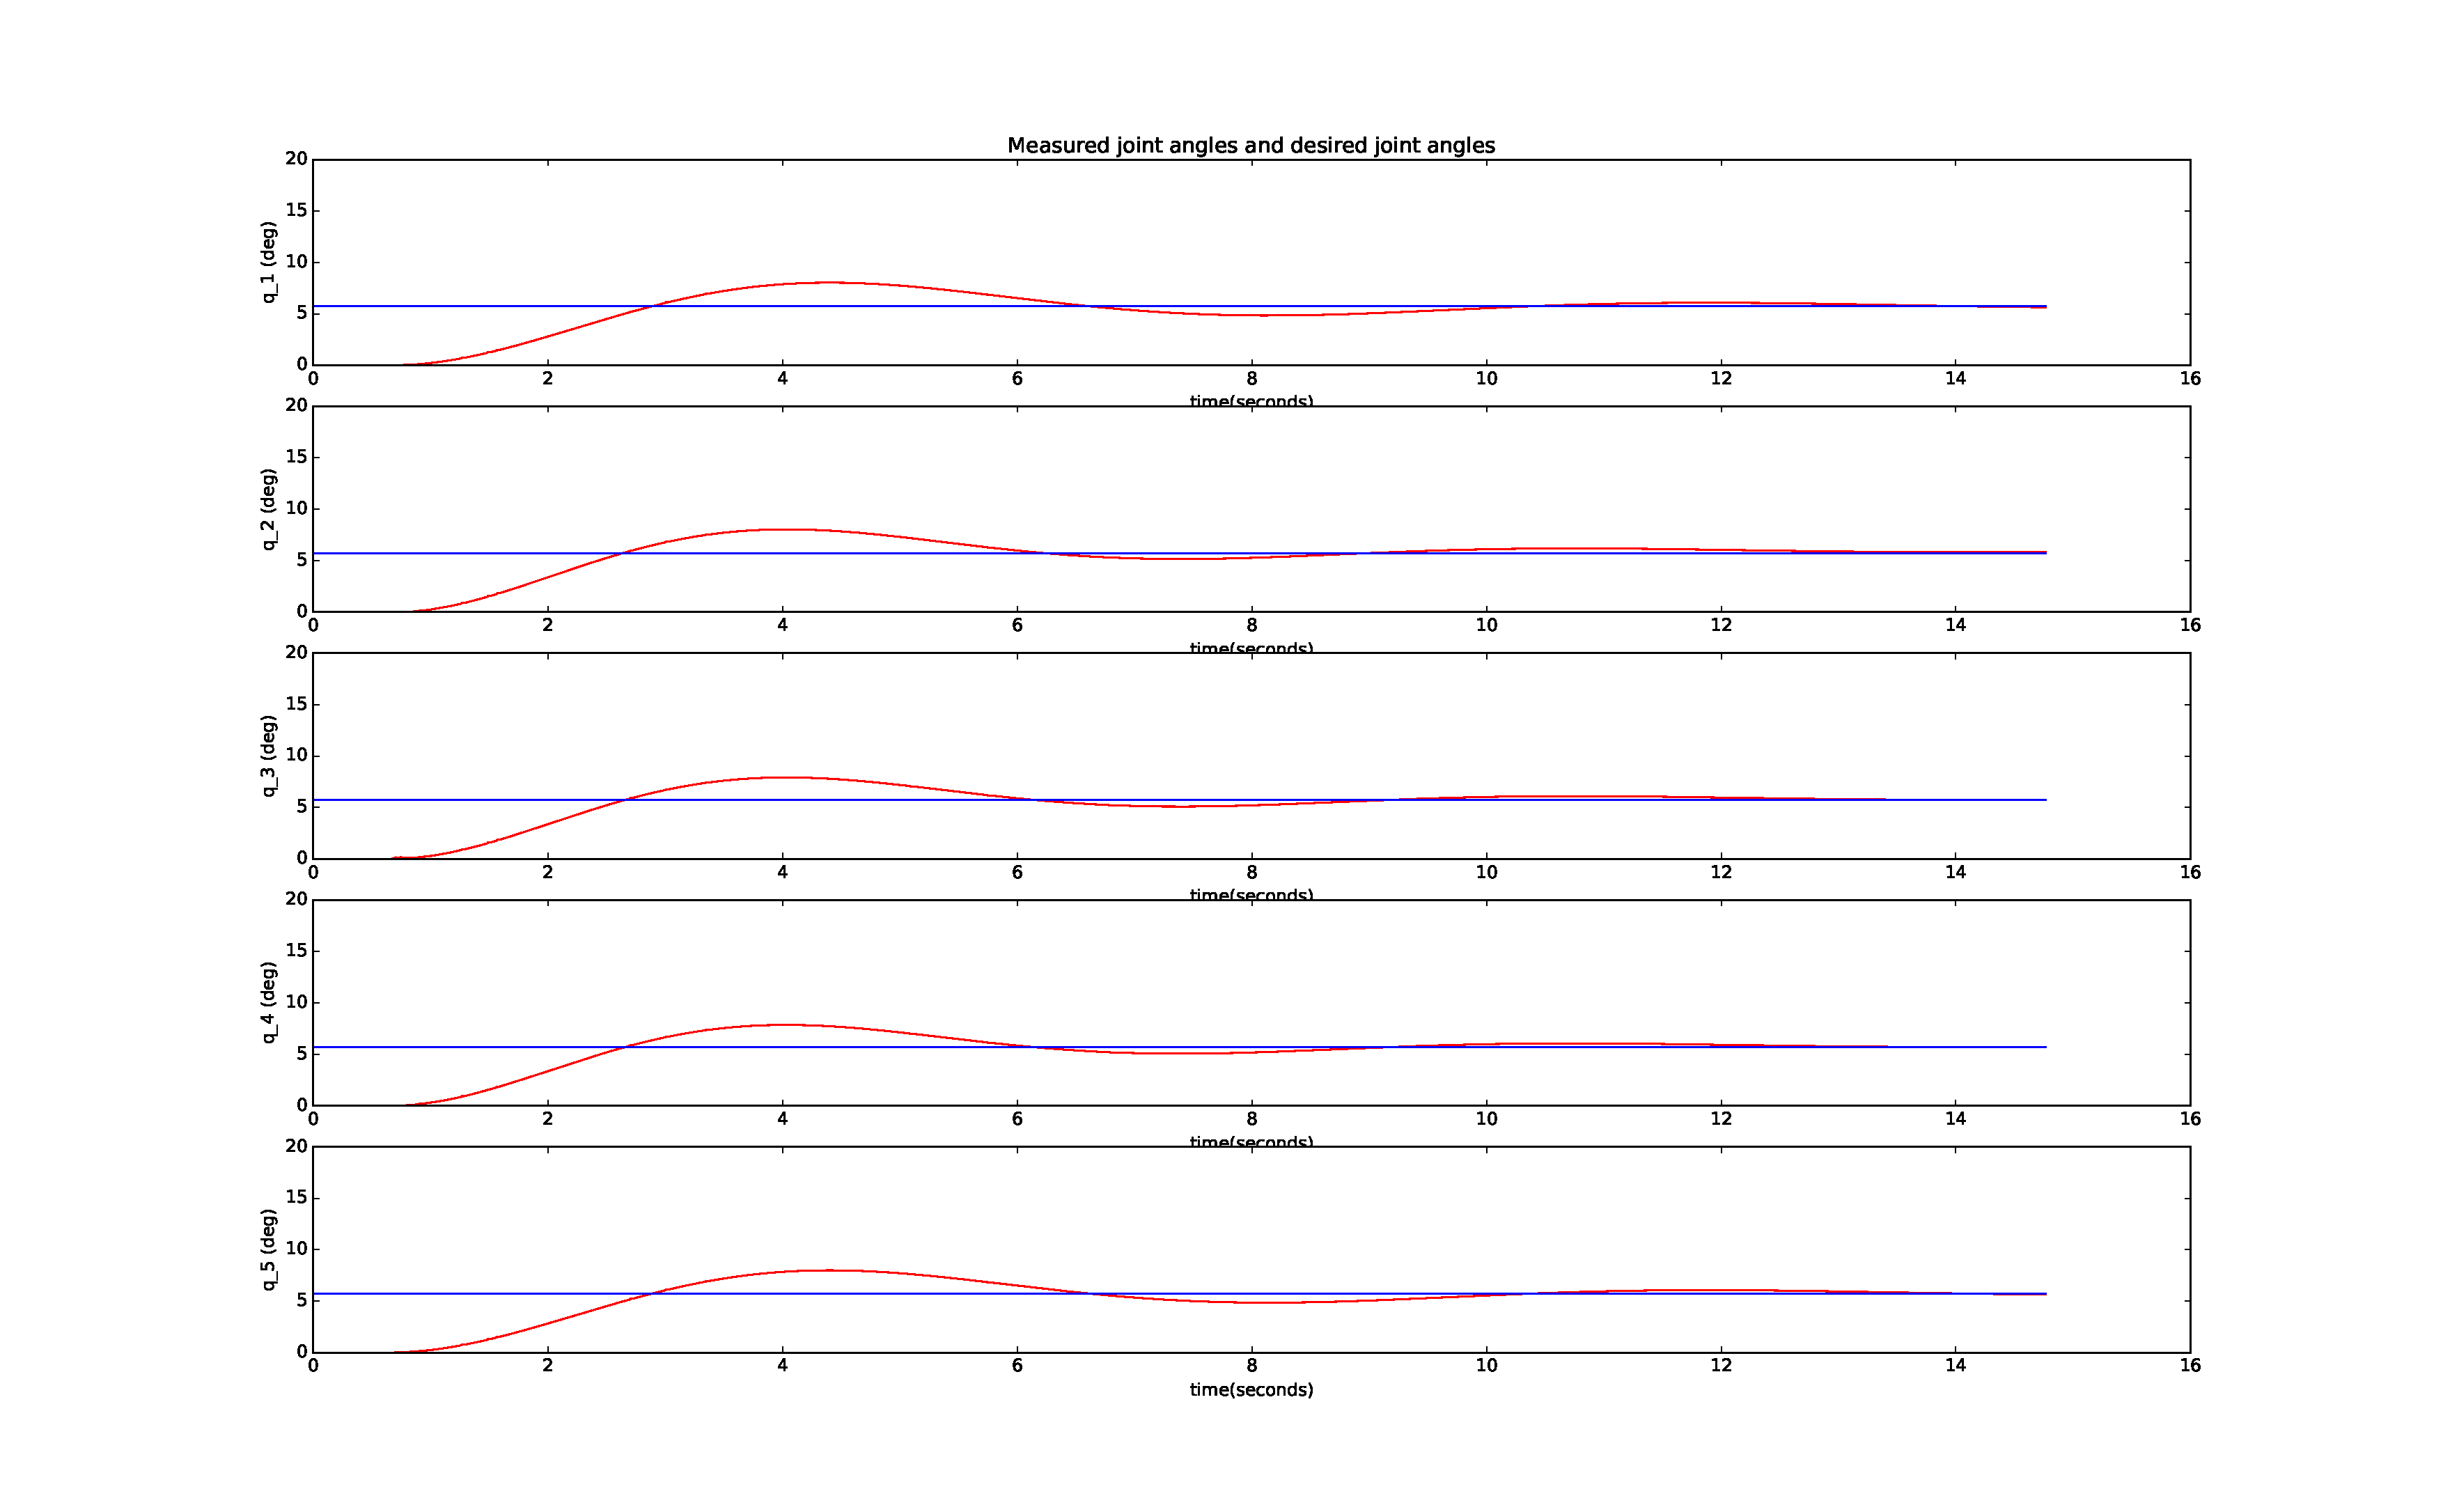
\includegraphics[width=.9\textwidth]{img/joingangKp2.eps}
  \caption{}
  \label{fig:testkp2}
\end{figure}

\subsection*{Spline - interpolation}
The next step now is to make a spline to make more setpoints such that the steps are not so big. This can lead to better behaviour for the robot. 

\subsubsection*{Circle of acceptance}
One problem when calculating the next point is to jump to the next setpoint if all the joints has approached the same step or should it be individual steps such that all the joints settles at different time or all joint settles at the same time. 
